

\actTitle{Worksheet 4.1}


\noindent \textbf{Instructions:}  Work together in groups of  3 or 4 to complete the following problems.\\


\begin{enumerate}


\item Find a positive angle less than $360^\circ$ that is coterminal with the given angle.
\begin{enumerate}
\item  $\theta=400^\circ$\vfill
\item $\alpha=-160^\circ$\vfill
\vfill
\end{enumerate}


\item Find a positive angle less than $2\pi$ that is coterminal with the given angle.
\begin{enumerate}
\item  $\displaystyle \beta=-\frac{\pi}{15}$\vfill
\item $\displaystyle \phi=\frac{34\pi}{9}$\vfill
\vfill
\end{enumerate}

\item Find the radian measure of the central angle $\theta$ of a circle of radius $r=8$ meters that intercepts an arc of length $s=14$ meters.\vfill
\vfill
\newpage

\item The minute hand of a clock is 3 inches long.  How far does the tip of the minute hand move in 45 minutes?\vfill

\item The minute hand of a clock moves from 12:10 to 12:30.
\begin{enumerate}
\item How many degrees does it move during this time?\vfill
\item How many radians does it move during this time?\vfill
\item If the minute hand is 10 inches in length, determine the exact distance the tip of the minute hand travels during this time.\vfill
\end{enumerate}
\newpage

\item Find the exact area of the following sectors given the radius of the circle $r$ and the subtended angle $\theta$.  Then round the result to the nearest tenth of a unit.

\begin{enumerate}
\item $r=6$ m; $\theta=\frac{5\pi}{3}$\vfill
\item $r=1.2$ ft; $\theta=\frac{\pi}{6}$\vfill
\item $r=3$ cm; $\theta=120^\circ $\vfill

\end{enumerate}


\newpage

\item You are one member of a group of 8 friends who are going out for pizza.  A small pizza has a 6" radius, while a large pizza has 9"  radius.  Answer the following questions.
\begin{enumerate}
	\item How much pizza will each of you eat if you order two small pizzas?  Will you get more of less pizza if you order one large pizza? (Assume everyone eats the same amount and all the pizza is eaten.)
	\vfill
	\item How many inches of crust will each person eat if you order two smalls?  If you order one large will you get more crust?
	\vfill
	\item Suppose you and your friends want to order one pizza and that you each want to eat 50 square inches worth of pizza.  What should the radius of the pizza be?
	\vfill
\end{enumerate}

\newpage

\item Suppose that the three circles drawn below have radii of length 1, 2, and 3.  For each pair of points given below, find the shortest path connecting the points.
%\vspace{-1in}
\begin{center}
  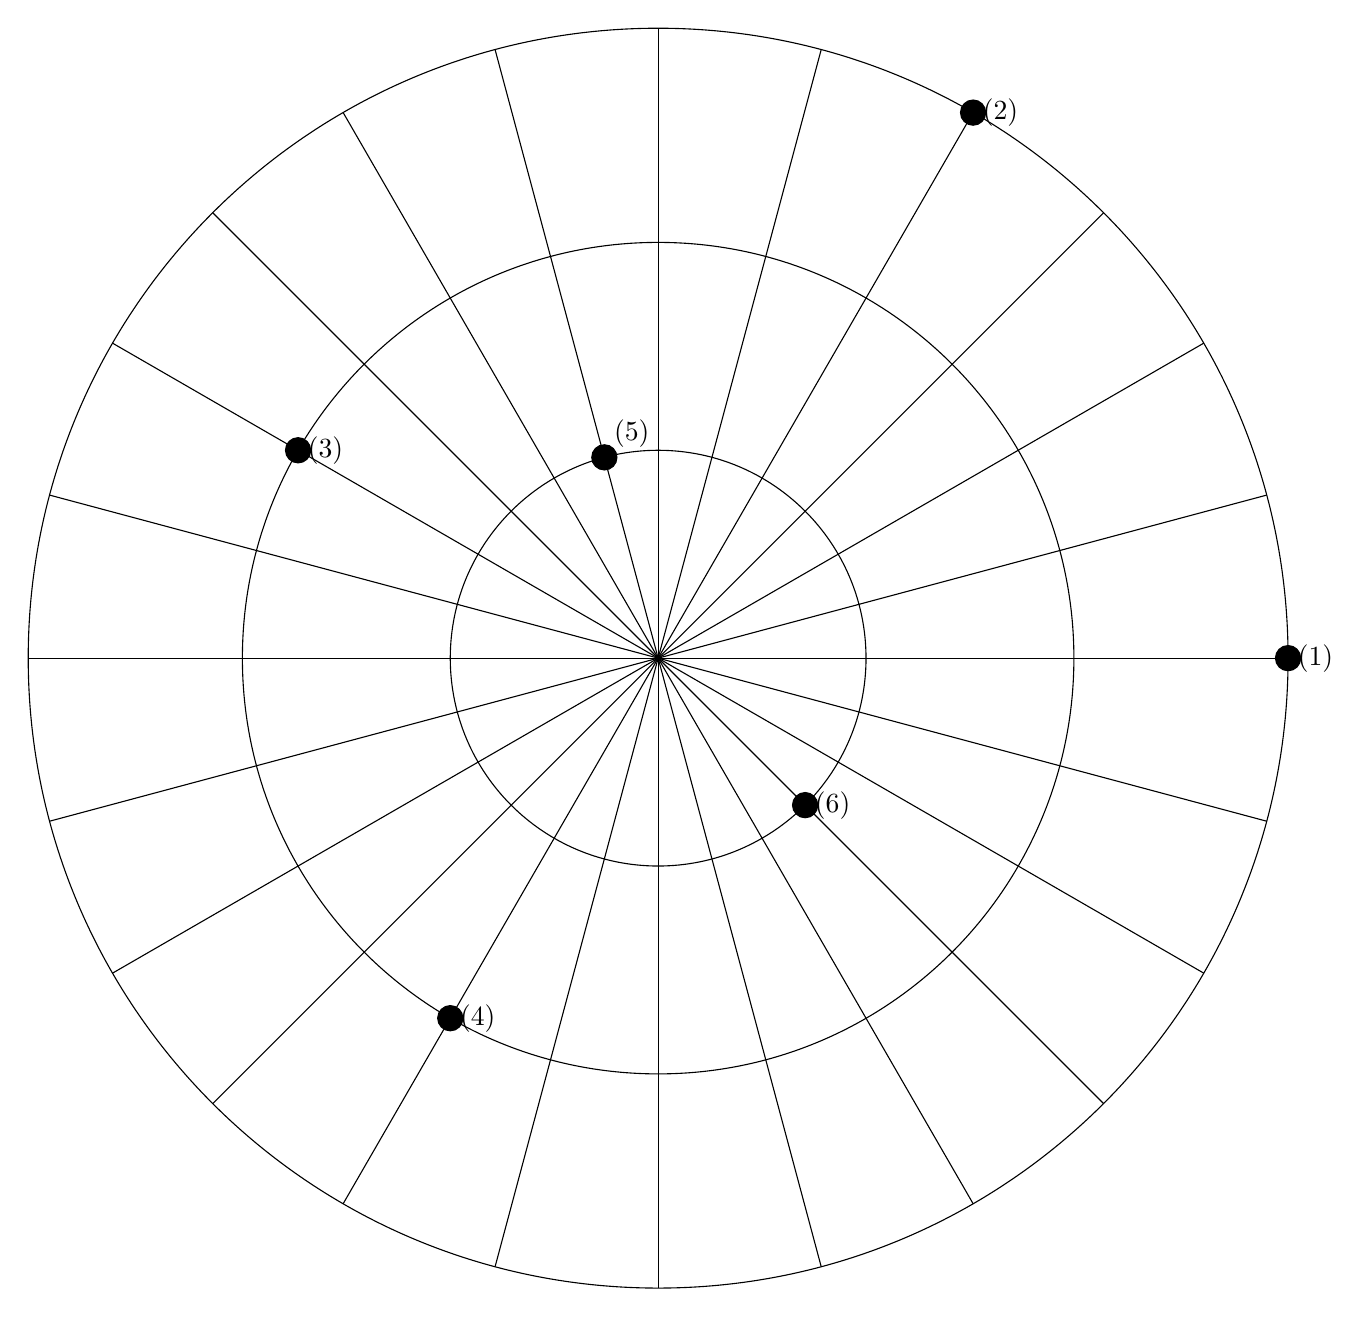
\begin{tikzpicture}[scale=8]
    \foreach \t in {0,15,30,...,345} {
      \draw[-] (0,0) -- (\t:1);
    }   
    \draw (0,0) circle(1);
    \draw (0,0) circle(0.66);
    \draw (0,0) circle(0.33);
    \filldraw[black] (1,0) circle (0.02) node[anchor=west] {(1)};
    \filldraw[black] (60:1) circle (0.02) node[anchor=west] {(2)};
    \filldraw[black] (150:0.66) circle (0.02) node[anchor=west] {(3)};
    \filldraw[black] (240:0.66) circle (0.02) node[anchor=west] {(4)};
    \filldraw[black] (105:0.33) circle (0.02) node[anchor=south west] {(5)};
    \filldraw[black] (315:0.33) circle (0.02) node[anchor=west] {(6)};
  \end{tikzpicture}
\end{center}



%\vspace{-1in}
\begin{enumerate}
\begin{multicols}{3}
	\item From (1) to (2).
	\item From (3) to (4).
	\item From (5) to (6).
	\item From (3) to (5).
	\item From (2) to (4), \\
	avoiding the center
\end{multicols}
\end{enumerate}




\end{enumerate}

